This section provides an overview of MFIX-Exa's Discrete Element Modelling (DEM)
abilities. MFIX-Exa's DEM simulations retain all the functionality of MFIX-DEM. 
MFIX-Exa can be run in both a pure granular (particles only) mode  
as well as a particle fluid-coupling mode. In the latter case, MFIX-Exa models 
the fluid phase as a continuum and models the
particles of the solid phase individually. This approach supports a wide range 
of customization for particle dynamics, including mutliple particle collision 
force and drag schemes. For more information on the DEM capabilities of MFIX-Exa
see \demdoc\ on the MFIX Documentation webpage 
{\url{https://mfix.netl.doe.gov/download/mfix/mfix_current_documentation/dem_doc_2012-1.pdf}}.

\section{Overview}

\begin{figure}
    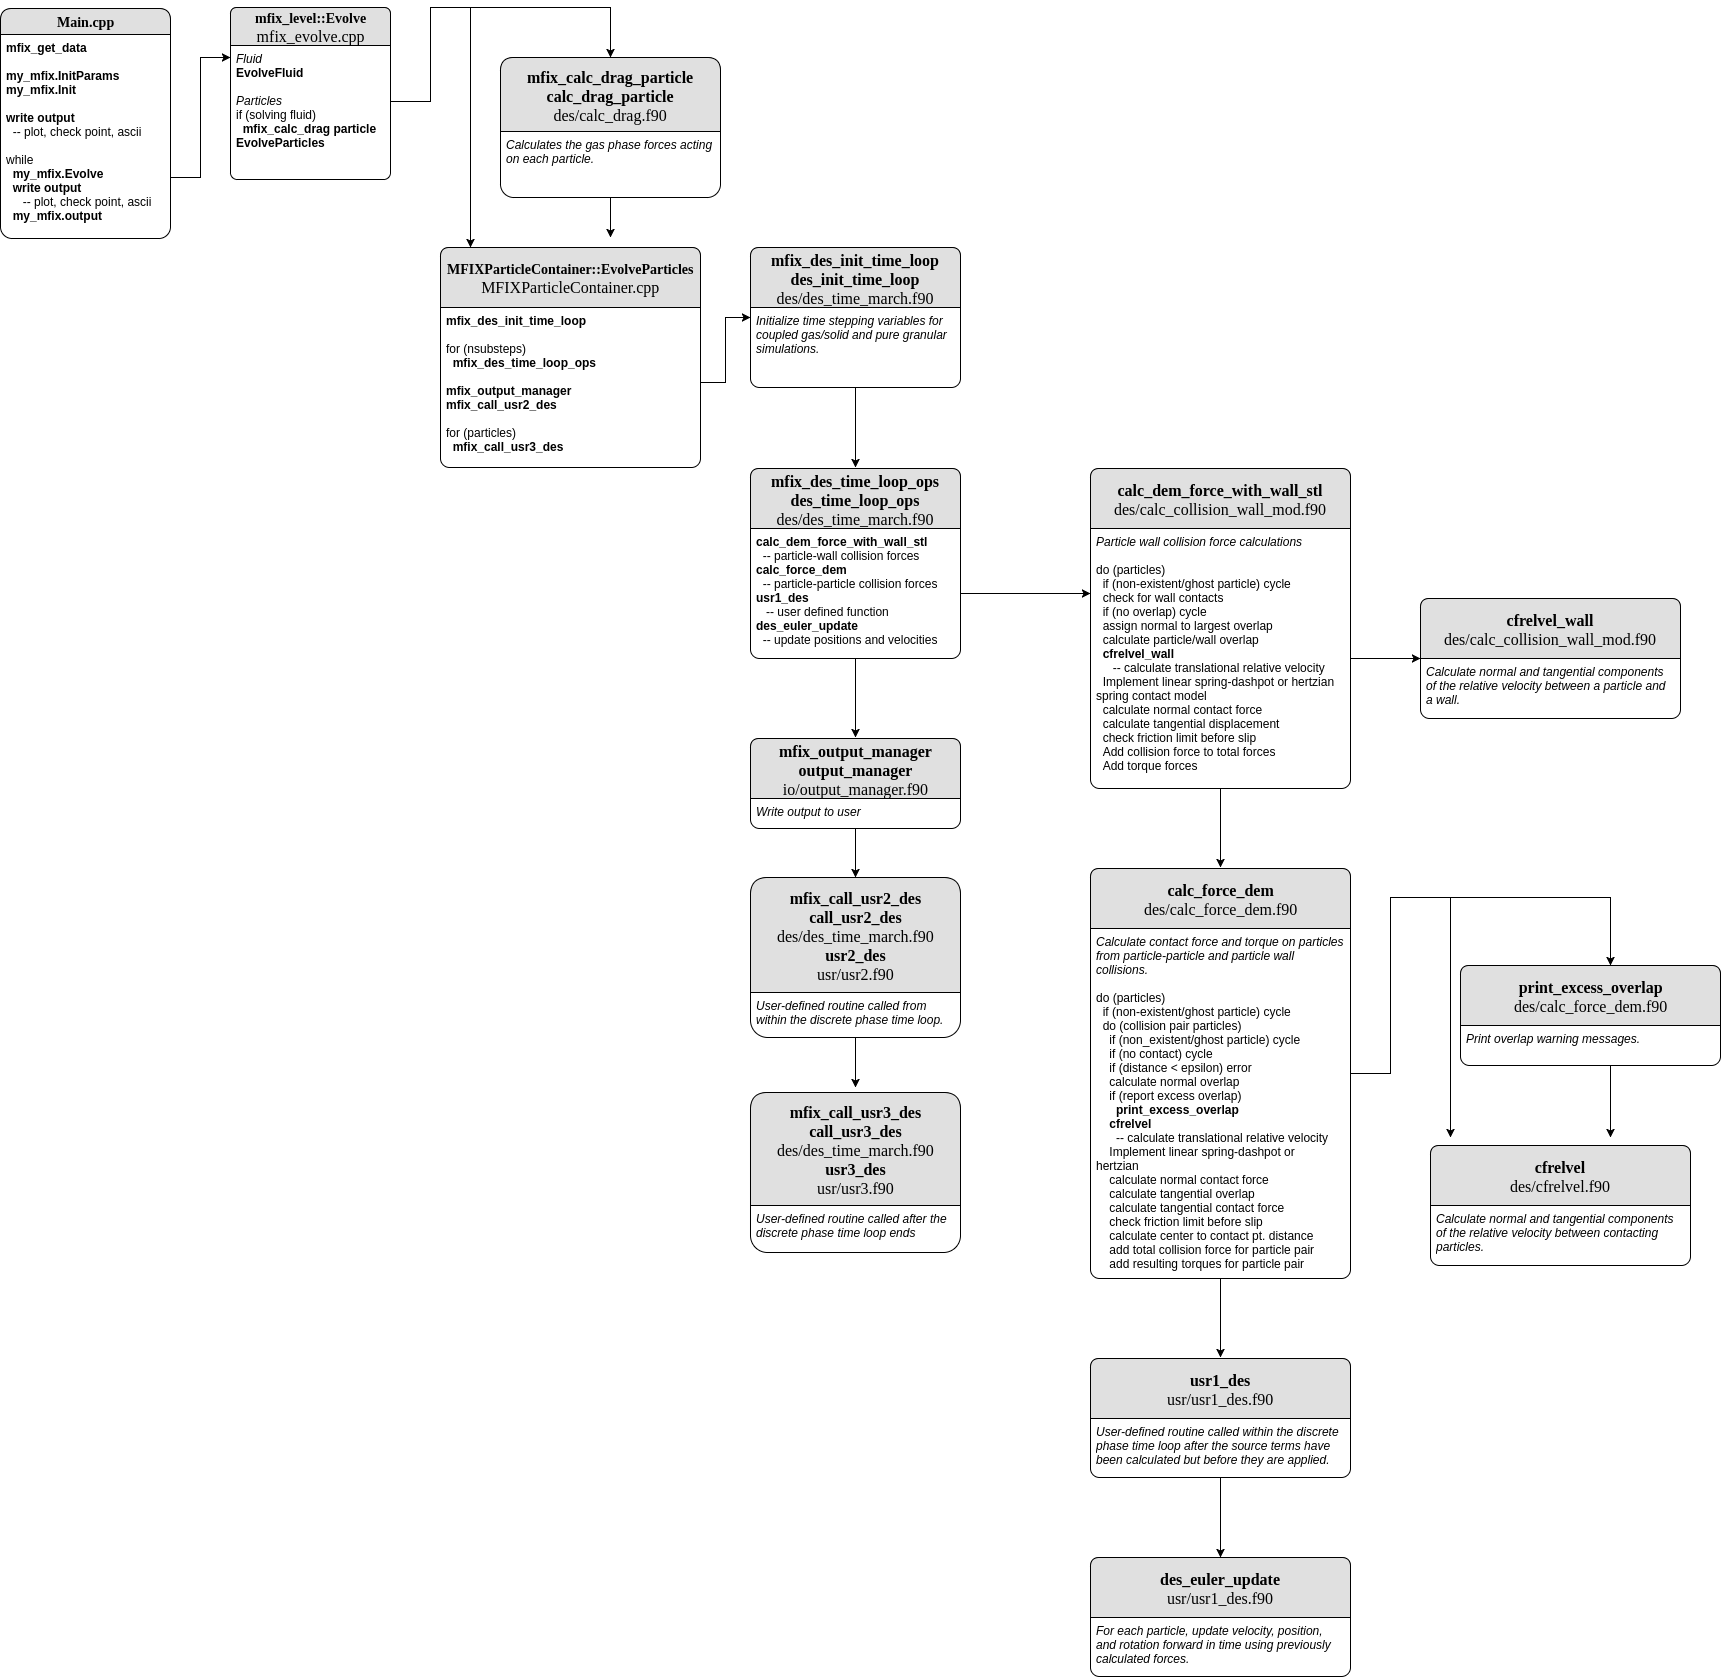
\includegraphics[width=\linewidth,natwidth=800, natheight=600]{./Particles/MFIX-Particle-Diagram.png} 
    \caption{Particle Routines Flowchart}
    \label{fig:pflowchart}
\end{figure}

\mfix\ retains all the functionality of MFIX-DEM. A detailed discription of the
particles dynamics and thus be found in \demdoc.
In addition, figure \ref{fig:pflowchart} provides a visual representation
of the particle routines in \mfix. 

\section{Equations}

If we define ${\mathbf x}_i$ and ${\bf u}_i$ as the location and velocity of particle $i$, respectively, then we wish
to solve
\begin{eqnarray}
\frac{d {\mathbf x}_i}{d t} &=& \frac{1}{a} {\mathbf u}_i \\
\frac{d (a {\mathbf u}_i) }{d t} &=& {\mathbf g}_i
\end{eqnarray}
where ${\mathbf g}_i$ is the gravitational force evaluated at the location of particle $i$, i.e., 
${\mathbf g}_i = {\mathbf g}({\mathbf x}_i,t).$

\section{Initializing the Particles}

\noindent There are several different ways in which particles can currently be initialized:

\subsection{Read from an ASCII file}

To enable this option, set \\

\noindent {\bf mfix.particle\_init\_type = AsciiFile} \\
\noindent {\bf mfix.ascii\_particle\_file =}{\em particle\_file}

Here {\em particle\_file} is the user-specified name of the file.  The first line in this file is
assumed to contain the number of particles.  Each line after that contains  \\

x y z mass xdot ydot zdot \\

Note that the variable that we call the particle velocity, ${\mathbf u} = a {\bf \dot{x}}$, 
so we must multiply ${\bf \dot{x}}$, by $a$ when we initialize the particles.

\subsection{Read from a binary file}

To enable this option, set \\

\noindent {\bf mfix.particle\_init\_type = BinaryFile} \\
\noindent {\bf mfix.binary\_particle\_file =}{\em particle\_file} \\

As with the ASCII read, the first line in this file is
assumed to contain the number of particles.  Each line after that contains  \\

x y z mass xdot ydot zdot \\

Note that the variable that we call the particle velocity, ${\mathbf u} = a {\bf \dot{x}}$, 
so we must multiply ${\bf \dot{x}}$, by $a$ when we initialize the particles.

\subsection{Read from a binary "meta" file}

This option allows you to read particles from a series of files rather than 
just a single file.   To enable this option, set \\

\noindent {\bf mfix.particle\_init\_type = BinaryMetaFile} \\
\noindent {\bf mfix.binary\_particle\_file =}{\em particle\_file} \\

In this case the {\em particle\_file} you specify is an ASCII file specifying a
list of file names with full paths.   Each of the files in this list is assumed
to be binary and is read sequentially (individual files are read in parallel) in 
the order listed.

\subsection{Reading SPH particles}

For some applications it is useful to initialize the grid data with SPH-type
particles.   To enable this option, you must set \\

\noindent {\bf mfix.do\_santa\_barbara = 1} \\
\noindent {\bf mfix.init\_with\_sph\_particles = 1} \\

\noindent The SPH-type particles can then be read in by setting \\

\noindent {\bf mfix.sph\_particle\_file =}{\em sph\_particle\_file} \\

\noindent where {\em sph\_particle\_file} is the user-specified name of the file
containing the SPH particles.  The type of {\em sph\_particle\_file} 
must be the same (Ascii, Binary or BinaryMeta) as the dark matter particle 
file as specified by   \\

\noindent {\bf mfix.particle\_init\_type = } \\

\noindent The SPH particles will be discarded by the code once the grid data has been initialized.

\subsection{Random placement}

To enable this option, set \\

\noindent {\bf mfix.mfix.particle\_init\_type = Random} \\

\noindent There are then a number of parameters to set, for example: \\

\noindent {\bf mfix.particle\_initrandom\_count = 100000}

\noindent {\bf mfix.particle\_initrandom\_mass  = 1}

\noindent {\bf mfix.particle\_initrandom\_iseed = 15}

\subsection{Cosmological}

Using cosmological initial conditions is a three step process:
\begin{enumerate}
	\item Generating a transfer function (e.g. with \texttt{camb})
	\item Generating an initial displacement field (with \texttt{mfix-ic})
	\item Starting mfix
\end{enumerate}

In the following we will look at each step a bit closer.

\subsubsection{Generating a transfer function}

	The transfer function is used in \texttt{mfix-ic} to generate the power
	spectrum. The usual way is to use \texttt{camb}\footnote{See \url{http://camb.info/}}
	to calculate it for the desired universe. A sample \texttt{camb.ini} is
	provided with \texttt{mfix-ic}. The important options are: 
	\begin{itemize}
		\item {\bf transfer\_redshift(1) = 50}
		\item {\bf transfer\_matterpower(1) = tf} 		
	\end{itemize}

	which determine the initial time for the simulation. You should make sure
	that you catch all necessary wave numbers for the considered box length and
	resolution.
	
	From the \texttt{camb} output you have to note values for \texttt{sigma\_8}
	for a redshift of zero and the initial redshift. We need this to compute
	the right normalization.
	
\subsubsection{Setting up the initial displacements}
	
	We calculate the initial displacements with a stand-alone program called
	\texttt{mfix-ic}. This takes a transfer function and some cosmological parameters
	as an argument and outputs an "init" directory which basically contains initial
	displacements for every grid point in an AMReX MultiFAB. Furthermore the mf 
	contains a fourth field containing the density contrast as initial condition
	for the baryonic matter. \\
	\texttt{mfix-ic} is started with an ``inputs``
	file similar to the one from MFIX-Exa. A sample one is provided. The options are
\begin{verbatim}
#Omega_{Matter}
cosmo.omegam = 0.272
#Omega_{Lambda}
cosmo.omegax = 0.728

#equation of state paramater omega_{effective}
cosmo.weff = -0.980

#Omega_{baryon}*Hubble^2 
cosmo.ombh2 = 0.0226
#Hubble/100km/s
cosmo.hubble = 0.704
#scalar spectral index
cosmo.enn = 0.963
# initial z
cosmo.z_init = 50

#sidelength of the box (in Mpc)
cosmo.boxside = 90.14
#seed of the rng
cosmo.isd = 100
#resolution of the box
cosmo.gridpoints = 256
#the output file name
cosmo.initDirName = init

#choose the source of the transferfunction
cosmo.transferfunction = CAMB

#some tabulated transferfunction generated with camb (compare camb-ini-file)
cosmo.tabulatedTk = tf
# sigma8 for the input tf at z=0 and initial z (to calc the growthfactor)
cosmo.init_sigma8_0 = 0.7891368
cosmo.init_sigma8_init = 2.0463364E-02
\end{verbatim} 

	The code solves the equation
	\begin{align}
	P(k,a) = 2\pi^2\delta^2_H \frac{k^n}{H_0^{n+3}}T^2(k)\left( \frac{D(a)}{D(a=1)} \right)^2
	\end{align}
	to calculate $P$ and from that gaussian distributed density perturbations
	$\delta$ following that spectrum. Particle displacements are then calculated
	as Zel'dovich displacements.
	
	Non-gaussian effects as well as neutrino contributions are planned for the
	future.
	
\subsubsection{Using MFIX-Exa with cosmological initial conditions}
	\begin{itemize}
		\item {\bf mfix.mfix.particle\_init\_type = Cosmological} \\ 
			set the \emph{right} init type
		\item {\bf cosmo.initDirName = init} \\
			set the name of the displacements directory (AMReX format)
		\item {\bf cosmo.particle\_mass = 0.19178304E+10} \\
			sets the mass [$M_\odot$] of each particle
		\item {\bf cosmo.omegam = 0.272} \\
			set $\Omega_{Matter}$
		\item {\bf cosmo.omegax = 0.728} \\
			set $\Omega_\Lambda$
		\item {\bf cosmo.hubble = 0.704} \\
			set the reduced hubble constant $h$
	\end{itemize}
	
	We will generate a particle of mass \textbf{particle\_mass} in every grid cell
	displaced from the center by the value found in the \textbf{initDirName} for
	that cell. Velocities are calculated in the Zel'dovich approximation by
	\begin{align}
		\vec{v} = \Delta{\vec{x}} \times 100 \text{km/s} \times a \sqrt{\Omega_M/a^3+\Omega_\Lambda} \times L_{\text{box}}
	\end{align}
	where $\Delta{\vec{x}}$ is the displacement of the particle.
	
\section{Time Stepping}

\noindent There are currently two different ways in which particles can be moved:

\subsection{Random}

\noindent To enable this option, set \\

\noindent {\bf mfix.particle\_move\_type = Random} \\

\noindent Update the particle positions at the end of each coarse time step using a 
random number between 0 and 1 multiplied by 0.25 dx.

\subsection{Motion by Self-Gravity}

\noindent To enable this option, set \\

\noindent {\bf mfix.particle\_move\_type = Gravitational} \\

\subsubsection{Move-Kick-Drift Algorithm}

In each time step:
\begin{itemize}
\item Solve for ${\mathbf g}^n$  (only if multilevel, otherwise use ${\mathbf g}^{n+1}$ from previous step)
\item ${\mathbf u}_i^{\nph} = \frac{1}{a^{\nph}} ( (a^n {\mathbf u}^n_i) + \frac{\dt}{2} \; {\mathbf g}^n_i )$
\item ${\mathbf x}_i^{n+1 } = {\mathbf x}^n_i +  \frac{\dt}{a^{\nph}}  {\mathbf u}_i^{\nph}$
\item Solve for ${\mathbf g}^{n+1}$ using ${\mathbf x}_i^{n+1}$
\item ${\mathbf u}_i^{n+1} = \frac{1}{a^{n+1}} ( (a^{\nph} {\mathbf u}^{\nph}_i) + \frac{\dt}{2} \; {\mathbf g}^{n+1}_i )$
\end{itemize}

Note that at the end of the timestep ${\bf x}_i^{n+1}$ is consistent with ${\bf g}^{n+1}$ becasue
we have not advanced the positions after computing the new-time gravity.  This has the benefit that
we perform only one gravity solve per timestep (in a single-level calculation with no hydro) because
the particles are only moved once.

\subsubsection{Computing {\bf g}}

We solve for the gravitational vector as follows:
\begin{itemize}
\item Assign the mass of the particles onto the grid in the form of density, $\rho_{DM}$.  
The mass of each particle is assumed to be uniformly distributed over a cube of side $\Delta x$, 
centered at what we call the position of the particle.    We distribute the mass of each
particle to the cells on the grid in proportion to the volume of the intersection of each cell
with the particle's cube.   We then divide these cell values by $\Delta x^3$ so that the
right hand side of the Poisson solve will be in units of density rather than mass.  
Note that this is the {\it comoving} density.

\item Solve $\nabla^2 \phi = \frac{4 \pi G}{a} \rho_{DM}$.
We discretize with the standard 7-point Laplacian (5-point in 2D) 
and use multigrid with Gauss-Seidel red-black relaxation to solve the equation for $\phi$ at cell centers.

\item Compute the normal component of ${\bf g} = -\nabla \phi$ at cell faces by differencing the adjacent values of $\phi,$
e.g. if $\gb = (g_x, g_y, g_z),$ then we define $g_x$ on cell faces with a normal in the x-direction by computing
$g_{x,i-\myhalf,j,k} = -(\phi_{i,j,k} - \phi_{i-1,j,k}) / \Delta x.$

\item  Interpolate each component of ${\bf g}$ from normal cell faces onto each particle position using 
linear interpolation in the normal direction.

\end{itemize}

%\subsection{Predictor-Corrector}
%
%An alternative to the above algorithm would be the following predictor-corrector approach:
%
%\begin{itemize}
%\item Solve for ${\bf g}^n$
%\item ${\bf v}_i^{n+1,*} = {\bf v}^n_i + \dt \; {\bf g}^n$
%\item ${\bf x}_i^{n+1,*} = {\bf x}^n_i + \dt \; {\bf v}_i^n$
%\item Solve for ${\bf g}^{n+1}$ using ${\bf x}_i^{n+1,*}$
%\item ${\bf v}_i^{n+1} = {\bf v}^{n+1,*}_i + \frac{\dt}{2} \; ({\bf g}^{n+1} - {\bf g}^n)$
%\item ${\bf x}_i^{n+1} = {\bf x}^{n+1,*}_i + \frac{\dt}{2} \; ({\bf v}_i^{n+1} - {\bf v}_i^n)$
%\end{itemize}
%
%\noindent This has two issues:
%\begin{itemize}
%\item First, the gravity at the end of the timestep is not consistent with the particle positions at the end of the timestep.
%Thus this will require an additional solve per timestep because we move the particles twice per timestep.
%\item Second, this increases the memory required per particle because we would need to keep both ${\bf v}^n_i$
%and ${\bf v}^{n+1,*}_i$ over the course of a timestep.
%\end{itemize}

\section{Output Format}

\subsection{Checkpoint Files}

The particle positions and velocities are stored in a binary file in each checkpoint directory.  
This format is designed for being read by the code at restart rather than for diagnostics. \\

We note that the value of $a$ is also written in each checkpoint directory, 
in a separate ASCII file called {\em comoving\_a}, containing only the single value. \\

\subsection{Plot Files}

If {\bf particles.write\_in\_plotfile =} 1 in the inputs file 
then the particle positions and velocities will be written in a binary file in each plotfile directory.  

In addition, we can also
visualize the particle locations as represented on the grid.  There are two ``derived quantities''
which represent the particles.  Setting \\

\noindent {\bf amr.derive\_plot\_vars = particle\_count particle\_mass\_density} \\
\noindent {\bf amr.plot\_vars = NONE} \\

\noindent in the inputs file will generate plotfiles with only two variables.  
{\bf particle\_count} represents the number of particles in a grid cell; 
{\bf particle\_mass\_density} is the density on the grid resulting from the particles.

We note that the value of $a$ is also written in each plotfile directory, 
in a separate ASCII file called {\em comoving\_a}, containing only the single value. \\

\subsection{ASCII Particle Files}

To generate an ASCII file containing the particle positions and velocities, 
one needs to restart from a checkpoint
file but doesn't need to run any steps.  For example, if chk00350 exists, then one can set: \\

\noindent {\bf amr.restart = chk00350} \\
\noindent {\bf max\_step = 350} \\
\noindent {\bf particles.particle\_output\_file =} {\em particle\_output} \\

\noindent which would tell the code to restart from chk00350, not to take any further time steps, and to write an ASCII-format 
file called {\em particle\_output}. \\

\noindent This file has the same format as the ASCII input file: \\

\noindent number of particles \\ 
x y z mass xdot ydot zdot \\

\subsection{Run-time Data Logs}

If you set \\

\noindent {\bf amr.data\_log = }{\em log\_file}  \\

\noindent in the inputs file, then at run-time the code will write a log file with entries every coarse
grid time step, containing \\

\noindent nstep  time   dt   redshift   a


\subsection{Run-time Screen Output}

There are a number of flags that control the verbosity written to the screen at run-time.  These are:

\noindent {\bf amr.v } \\
\noindent {\bf mfix.v } \\
\noindent {\bf gravity.v } \\
\noindent {\bf mg.v } \\
\noindent {\bf particles.v } \\

These control printing  about the state of the calculation (time, value of $a$, etc) as well as
timing information.
